\documentclass[aspectratio=169,10pt]{beamer}

% ============================================================
% Physics-informed and agentic AI for accelerating CFD
% Expanded deck (detailed explanations). Sources:
%   - classical physics-informed learning (from CFD_QAI.tex, quantum/hybrid removed)
%   - crystal-growth case study (from main_nerips.tex)
%   - agentic CFD / AutoFOAM (from presentation.tex)
%
% IMAGES: no images are embedded. Every figure is a dashed placeholder
% that shows the file name it expects. Put the PNG into  images/  with
% exactly that name and recompile -- the placeholder is replaced automatically.
% ============================================================
\usepackage[T1]{fontenc}
\usepackage[utf8]{inputenc}
\usepackage{lmodern}
\usepackage{amsmath,amssymb}
\usepackage{booktabs}
\usepackage{array}
\usepackage{tabularx}
\usepackage{graphicx}
\usepackage{xcolor}
\usepackage{hyperref}
\usepackage{tikz}
\usetikzlibrary{arrows.meta,positioning,fit,calc}
\graphicspath{{images/}}
\newcolumntype{L}{>{\raggedright\arraybackslash}X}

% ---------- colours ----------
\definecolor{navy}{HTML}{173B4D}
\definecolor{teal}{HTML}{2C6975}
\definecolor{mint}{HTML}{E9F4F2}
\definecolor{orange}{HTML}{D9822B}
\definecolor{lightorange}{HTML}{FBEBDA}
\definecolor{lightgray}{HTML}{F3F5F6}
\definecolor{midgray}{HTML}{68757A}
\definecolor{dark}{HTML}{1F2528}
\definecolor{alertred}{HTML}{B5473A}

\setbeamercolor{normal text}{fg=dark,bg=white}
\setbeamercolor{structure}{fg=teal}
\setbeamercolor{frametitle}{fg=navy,bg=white}
\setbeamercolor{title}{fg=navy}
\setbeamercolor{footline}{fg=midgray,bg=white}
\setbeamercolor{block title}{fg=white,bg=navy}
\setbeamercolor{block body}{fg=dark,bg=lightgray}
\setbeamercolor{block title alerted}{fg=white,bg=orange}
\setbeamercolor{block body alerted}{fg=dark,bg=lightorange}
\setbeamercolor{block title example}{fg=white,bg=teal}
\setbeamercolor{block body example}{fg=dark,bg=mint}

\setbeamerfont{frametitle}{size=\large,series=\bfseries}
\setbeamerfont{block title}{size=\small,series=\bfseries}
\setbeamertemplate{navigation symbols}{}
\setbeamertemplate{itemize item}{\color{teal}\small$\blacktriangleright$}
\setbeamertemplate{itemize subitem}{\color{orange}\scriptsize$\blacktriangleright$}
\setbeamertemplate{section in toc}[sections numbered]
\setbeamercolor{section in toc}{fg=navy}

% ---------- frame title: small section tag + title + accent rule ----------
\setbeamertemplate{frametitle}{
  \vspace{0.12cm}
  \begin{beamercolorbox}[wd=\paperwidth,leftskip=0.65cm,rightskip=0.65cm]{frametitle}
    {\fontsize{7}{8}\selectfont\color{orange}\bfseries\MakeUppercase{\insertsection}\par}
    \vspace{0.02cm}
    \usebeamerfont{frametitle}\insertframetitle\par
    \vspace{0.03cm}
    {\color{orange}\rule{0.65cm}{1.6pt}}
  \end{beamercolorbox}
}

% ---------- footer ----------
\setbeamertemplate{footline}{
  \leavevmode
  \hbox{
    \begin{beamercolorbox}[wd=.82\paperwidth,ht=0.35cm,dp=0.15cm,leftskip=.65cm]{footline}
      \scriptsize Physics-informed and agentic AI for accelerating CFD
    \end{beamercolorbox}
    \begin{beamercolorbox}[wd=.18\paperwidth,ht=0.35cm,dp=0.15cm,rightskip=.65cm plus1fil]{footline}
      \scriptsize\insertframenumber
    \end{beamercolorbox}
  }
}

% ---------- helper macros ----------
\newcommand{\source}[1]{\vspace{0.05cm}{\scriptsize\color{midgray}Source: #1}}
\newcommand{\smallnote}[1]{{\scriptsize\color{midgray}#1}}
\newcommand{\key}[1]{\textcolor{teal}{\textbf{#1}}}
\newcommand{\highlight}[1]{\textcolor{orange}{\textbf{#1}}}

% \figbox{file-name-without-.png}{width}{height}{short description}
% If images/<file-name>.png exists it is inserted; otherwise a dashed placeholder is drawn.
\newcommand{\figbox}[4]{%
  \IfFileExists{images/#1.png}{%
    \includegraphics[width=#2,height=#3,keepaspectratio]{images/#1.png}%
  }{%
    \begin{tikzpicture}
      \node[draw=midgray,dashed,thick,fill=lightgray,minimum width=#2,minimum height=#3,
            align=center,text=midgray,font=\scriptsize,inner sep=3pt,text width=#2-6pt]
        {\textbf{[IMAGE PLACEHOLDER]}\\[1pt]\texttt{images/#1.png}\\[1pt]\textit{#4}};
    \end{tikzpicture}%
  }%
}

% ---------- title data ----------
\title{Physics-Informed and Agentic AI\\for Accelerating CFD Simulations}
\author{A Seshaditya}
\institute{QuaSi}
\date{}

% extra helper: small labelled equation box
\newcommand{\eqbox}[1]{\begin{center}\colorbox{mint}{\parbox{0.92\linewidth}{\centering #1}}\end{center}}
\begin{document}

% ============================================================ TITLE
\begin{frame}[plain]
  \begin{tikzpicture}[remember picture,overlay]
    \fill[navy] (current page.south west) rectangle (current page.north east);
    \fill[teal] (current page.south east) rectangle ([xshift=-0.20\paperwidth]current page.north east);
    \fill[orange] ([xshift=-0.20\paperwidth]current page.south east) rectangle ([xshift=-0.195\paperwidth]current page.north east);
  \end{tikzpicture}
  \vspace{0.9cm}
  \begin{minipage}[t][0.78\textheight]{0.74\textwidth}
    \raggedright
    {\color{white}\fontsize{22}{27}\selectfont\bfseries Physics-Informed and\\Agentic AI for Accelerating\\CFD Simulations\par}
    \vspace{0.45cm}
    {\color{white!80}\large From PINNs and neural operators\\to autonomous OpenFOAM workflows\par}
    \vfill
    {\color{white}\large A Seshaditya\\[1mm]QuaSi\par}
  \end{minipage}
\end{frame}

% ============================================================ AGENDA
\begin{frame}{Agenda}
  \begin{columns}[T,onlytextwidth]
    \column{0.52\textwidth}
    \vspace{0.2cm}
    \tableofcontents[hideallsubsections]
    \column{0.44\textwidth}
    \begin{block}{Storyline}
      \small
      CFD is accurate but costly $\rightarrow$ physics-informed models reduce the cost
      $\rightarrow$ agentic automation removes the set-up barrier $\rightarrow$ both need
      rigorous validation.
    \end{block}
    \begin{block}{Two bottlenecks, two tools}
      \small
      \textbf{Compute cost} of many simulations $\Rightarrow$ physics-informed surrogates.\\
      \textbf{Set-up expertise} for each simulation $\Rightarrow$ agentic case generation.
    \end{block}
  \end{columns}
\end{frame}

\begin{frame}{Glossary: terms used in this talk}
\small
\renewcommand{\arraystretch}{1.15}
\begin{tabularx}{\textwidth}{>{\bfseries}l L >{\bfseries}l L}
\toprule
CFD & Computational fluid dynamics: numerically solving fluid-flow equations. &
PDE & Partial differential equation, e.g.\ Navier--Stokes or heat equation.\\
PINN & Neural network trained so its output satisfies the PDE. &
Residual & How far a candidate solution is from satisfying the PDE at a point.\\
BC / IC & Boundary / initial conditions (values imposed at edges / at $t=0$). &
Autodiff & Automatic differentiation: exact derivatives of the network output.\\
Operator & Map from a function (input field) to a function (solution). &
NRMSE & RMSE divided by the standard deviation of the target field.\\
RANS & Reynolds-averaged Navier--Stokes (time-averaged turbulence model). &
OOD & Out-of-distribution: test cases never seen in training.\\
RAG & Retrieval-augmented generation (look up verified examples). &
SFT / DPO & Supervised fine-tuning / Direct Preference Optimisation.\\
\bottomrule
\end{tabularx}
\end{frame}

% ============================================================
\section{Motivation}
% ============================================================

\begin{frame}{CFD is accurate, but expensive}
\begin{columns}[T,onlytextwidth]
\column{0.52\textwidth}
\begin{block}{Why accelerate?}
\begin{itemize}\footnotesize
  \item \textbf{High cost per simulation:} high-fidelity, multi-physics CFD needs fine meshes and long runs.
  \item \textbf{The real cost is the sweep, not one run:} design studies vary pull rate, rotation rates, thermal boundary conditions, geometry\ldots{} each point is a new simulation.
  \item \textbf{Multi-physics coupling} (flow + heat + particles) adds model complexity.
  \item \textbf{Set-up expertise:} a valid case needs deep solver knowledge.
\end{itemize}
\end{block}
\vspace{0.1cm}
{\small\key{Goal:} keep the governing physics, cut the cost, and make set-up accessible.}

\column{0.45\textwidth}
\centering
\figbox{cz-process-schematic}{\linewidth}{3.8cm}{Silicon crystal-growth (CZ) process schematic: crucible, melt, crystal, rotation, heater}
\end{columns}
\end{frame}

\begin{frame}{Application focus: two demanding CFD settings}
\begin{columns}[T,onlytextwidth]
\column{0.49\textwidth}
\begin{block}{Silicon crystal growth (Czochralski, CZ)}
\begin{itemize}\small
  \item A seed crystal is pulled from molten silicon in a rotating crucible.
  \item Couples heat transfer, melt convection, pressure variation and rotating boundaries.
  \item The resulting thermal and flow fields largely determine crystal quality.
\end{itemize}
\end{block}
\centering
\figbox{cz-furnace-fields}{\linewidth}{2.5cm}{CZ melt flow / temperature field}

\column{0.49\textwidth}
\begin{block}{Cryogenic / hydrogen systems}
\begin{itemize}\small
  \item Design-oriented CFD for complex flow and thermal conditions.
  \item Faster surrogates support iterative design.
  \item Relevant to the wider space and energy use cases.
\end{itemize}
\end{block}
\centering
\figbox{cryogenic-system}{\linewidth}{2.5cm}{Cryogenic tank / hydrogen system CFD}
\end{columns}
\end{frame}

\begin{frame}{What the CFD has to solve (CZ melt)}
\begin{columns}[T,onlytextwidth]
\column{0.56\textwidth}
\begin{block}{Governing physics in the reference model}
\begin{itemize}\small
  \item Incompressible Navier--Stokes: momentum + continuity.
  \item Energy equation for temperature $T$.
  \item \textbf{Boussinesq buoyancy}: density varies with $T$ only in the buoyancy term, which drives natural convection.
  \item \textbf{Rotation:} crystal and crucible walls impose azimuthal velocity $u_\theta=\omega r$.
\end{itemize}
\end{block}
\begin{block}{Unknowns per point $(r,z)$}
\small $u_r,\;u_z,\;u_\theta$ (velocity), $p$ (pressure), $T$ (temperature): five coupled fields.
\end{block}
\column{0.40\textwidth}
\centering
\figbox{cz-domain-bcs}{\linewidth}{4.9cm}{2D axisymmetric melt domain with boundary conditions: rotating walls, slip free surface, hot wall, crucible bottom}
\end{columns}
\end{frame}

\begin{frame}{The technical story}
\centering
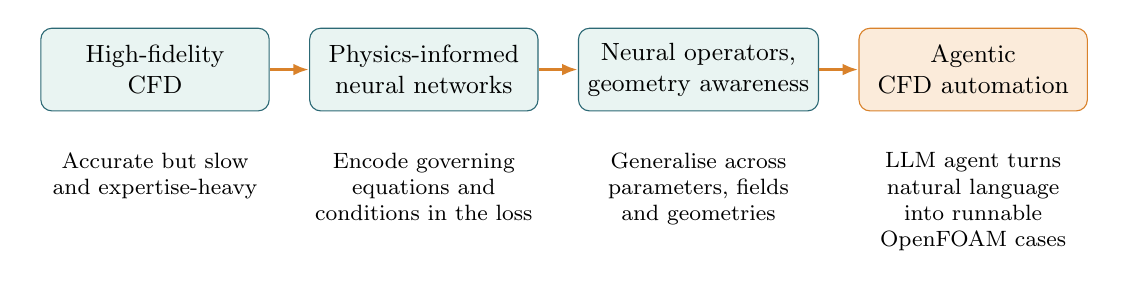
\begin{tikzpicture}[
  node distance=0.5cm,
  box/.style={rounded corners,draw=teal,fill=mint,minimum width=2.9cm,minimum height=1.05cm,align=center,font=\small},
  arr/.style={-{Latex[length=2mm]},very thick,draw=orange}
]
\node[box] (cfd) {High-fidelity\\CFD};
\node[box,right=of cfd] (pinn) {Physics-informed\\neural networks};
\node[box,right=of pinn] (op) {Neural operators,\\geometry awareness};
\node[box,right=of op,fill=lightorange,draw=orange] (ag) {Agentic\\CFD automation};
\draw[arr] (cfd)--(pinn); \draw[arr] (pinn)--(op); \draw[arr] (op)--(ag);
\node[below=0.4cm of cfd,align=center,text width=3.0cm,font=\footnotesize]{Accurate but slow and expertise-heavy};
\node[below=0.4cm of pinn,align=center,text width=3.0cm,font=\footnotesize]{Encode governing equations and conditions in the loss};
\node[below=0.4cm of op,align=center,text width=3.0cm,font=\footnotesize]{Generalise across parameters, fields and geometries};
\node[below=0.4cm of ag,align=center,text width=3.0cm,font=\footnotesize]{LLM agent turns natural language into runnable OpenFOAM cases};
\end{tikzpicture}

\vfill
\key{Research question:} how can physics-aware surrogates and autonomous case generation
together make CFD faster and more accessible, without losing physical validity?
\end{frame}

% ============================================================
\section{Physics-informed learning}
% ============================================================

\begin{frame}{Physics-Informed Neural Networks (PINNs): the idea}
\begin{columns}[T,onlytextwidth]
\column{0.50\textwidth}
\begin{block}{Core idea}
\footnotesize A neural network $\hat u_\theta(x,t)$ approximates the solution field. The loss penalises violations of the governing PDEs and of the boundary/initial conditions.
\end{block}
\begin{enumerate}\footnotesize
  \item Sample \textbf{collocation points} in the domain and on its boundary.
  \item Evaluate $\hat u_\theta$; obtain $\partial_t\hat u,\partial_x\hat u,\partial_{xx}\hat u,\dots$ by \textbf{automatic differentiation}.
  \item Form the PDE residual and BC/IC mismatch; minimise with Adam.
\end{enumerate}
\begin{itemize}\footnotesize
  \item Less dependence on large labelled datasets.
  \item Natural fit for multi-physics equations.
\end{itemize}
\source{\url{https://doi.org/10.1063/5.0226232}}

\column{0.46\textwidth}
\centering
\figbox{pinn-concept}{\linewidth}{3.6cm}{PINN concept: coordinates $\rightarrow$ network $\rightarrow$ field; autodiff gives residuals; loss = PDE + BC + IC}
\end{columns}
\end{frame}

\begin{frame}{PINN methodology: physics becomes part of the objective}
\begin{columns}[T,onlytextwidth]
\column{0.54\textwidth}
\[
L_{\mathrm{total}} = L_{\mathrm{PDE}} + L_{\mathrm{BC}} + L_{\mathrm{IC}} + \lambda L_{\mathrm{SAL}}
\]
\begin{description}\footnotesize
\item[$L_{\mathrm{PDE}}$] mean squared PDE residual at collocation points.
\item[$L_{\mathrm{BC}}$] mismatch with boundary conditions (e.g.\ $T=0$ at walls).
\item[$L_{\mathrm{IC}}$] mismatch with the initial state at $t=0$.
\item[$L_{\mathrm{SAL}}$] sensitivity-analysis term, with weighting factor $\lambda$.
\end{description}
\vspace{1mm}
\key{Computation:} derivatives come from automatic differentiation, so no mesh or finite-difference stencil is needed.\\[2pt]
\key{Key knob:} the \emph{relative weights} of these terms. The rest of this talk shows why they matter.

\column{0.43\textwidth}
\centering
\figbox{pinn-loss-diagram}{\linewidth}{4.0cm}{PINN loss composition / training workflow}
\end{columns}
\end{frame}

\begin{frame}{Why PINN training is not automatically stable}
\begin{columns}[T,onlytextwidth]
\column{0.52\textwidth}
\begin{block}{Known failure modes (prior work)}
\begin{itemize}\footnotesize
  \item \textbf{Optimisation stiffness:} PDE residual terms can make the landscape hard to navigate.
  \item \textbf{Gradient imbalance:} the loss term with the larger raw gradient dominates the update.
  \item \textbf{Competing loss terms:} fitting the PDE and the constraints are different goals.
\end{itemize}
\end{block}
\begin{alertblock}{Consequence}
\footnotesize A low \emph{total} loss can hide poor boundary satisfaction or weak physical consistency, and the failure is usually only found after the fact.
\end{alertblock}
\smallnote{Wang et al.\ 2021 (gradient pathologies); Krishnapriyan et al.\ 2021 (failure modes).}
\column{0.44\textwidth}
\begin{exampleblock}{Natural fix: adapt the loss weights}
\small
\begin{itemize}
  \item Normalise gradients of each term.
  \item Or adjust weights with a controller during training.
\end{itemize}
\vspace{2pt}
But adaptive weights change the objective itself, so \textbf{weighted totals are not comparable across methods}. This is exactly what the case study tests.
\end{exampleblock}
\end{columns}
\end{frame}

\begin{frame}{From PINNs to neural operators}
\begin{columns}[T,onlytextwidth]
\column{0.50\textwidth}
\begin{block}{Why move beyond a single solution?}
A PINN solves \emph{one} PDE instance and must be retrained when parameters change. Neural operators learn a mapping between \textbf{functions}: input field (coefficients, geometry, conditions) $\mapsto$ solution field.
\end{block}
\begin{itemize}\small
  \item \textbf{PINO}: physics-informed neural operators add the PDE residual to operator training.
  \item Targets \emph{families} of PDE solutions: one trained model, many parameter settings.
  \item Benefits: higher accuracy, multi-physics capability, data efficiency.
\end{itemize}
\column{0.46\textwidth}
\centering
\figbox{pino-architecture}{\linewidth}{5.2cm}{PINO / physics-informed operator: input function $\rightarrow$ operator network $\rightarrow$ solution function, with physics loss}
\end{columns}
\end{frame}

\begin{frame}{Geometry-aware operators: the next generalisation step}
\begin{columns}[T,onlytextwidth]
\column{0.50\textwidth}
\begin{block}{PI-GANO}
\footnotesize Physics-informed geometry-aware neural operator: generalises across PDE parameter representations \emph{and} across geometries, without retraining for each shape.
\end{block}
\source{arXiv:2408.01600v1}
\vspace{0.1cm}
\begin{block}{GAOT / MAGNO}
\footnotesize Geometry Aware Operator Transformer built on a multiscale attentional graph neural operator: attention-based operator learning on irregular meshes.
\end{block}
\source{arXiv:2505.18781v2}
\vspace{0.1cm}
{\footnotesize\key{Why it matters for CFD:} real design problems change the geometry, not only a scalar parameter.}
\column{0.46\textwidth}
\centering
\figbox{geometry-aware-operators}{\linewidth}{4.2cm}{PI-GANO / GAOT architecture overview}
\end{columns}
\end{frame}

\begin{frame}{Comparing the classical approaches}
\small
\renewcommand{\arraystretch}{1.1}
\begin{tabularx}{\textwidth}{>{\bfseries}l L L L}
\toprule
Approach & Primary idea & Strength & Open challenge \\
\midrule
PINN    & NN + PDE residuals          & Physics constraints, data efficiency & Training stability and scaling \\
PINO    & Operator learning + physics & Families of PDE solutions            & Generalisation across settings \\
PI-GANO & Geometry-aware operator     & Geometry generalisation              & Complex geometries / representations \\
GAOT    & Geometry-aware transformer  & Attention-based operator learning    & Computational cost and validation \\
\bottomrule
\end{tabularx}

\vspace{0.2cm}
\centering
\figbox{approach-comparison}{0.7\linewidth}{1.9cm}{Optional: comparison figure / benchmark chart}
\vfill
\raggedright\source{arXiv:2408.01600v1, arXiv:2505.18781v2.}
\end{frame}

% ============================================================
\section{Case study: crystal growth}
% ============================================================

\begin{frame}{Case study overview: two experiments, two questions}
\begin{columns}[T,onlytextwidth]
\column{0.48\textwidth}
\begin{block}{A. Adaptive PINN training}
\small
\textbf{Question:} when loss weights adapt during training, is a lower PDE loss really a better solution?\\[3pt]
Problems: (1) 1D heat equation with an analytical answer; (2) simplified Czochralski thermal-fluid PINN.\\[3pt]
Compared: Baseline PINN, GNPINN, AgenticPINN.
\end{block}
\column{0.48\textwidth}
\begin{block}{B. CFD surrogates (Gaussian process)}
\small
\textbf{Question:} how well does a surrogate predict a \emph{whole unseen operating condition}, field by field?\\[3pt]
Data: ANSYS Fluent reference CFD, three one-parameter sweeps.\\[3pt]
Metric: NRMSE per output field.
\end{block}
\end{columns}
\vspace{0.2cm}
\begin{alertblock}{Shared message}
\small Aggregate numbers hide where a model fails. Report component-level losses and field-wise errors.
\end{alertblock}
\vspace{0.1cm}
\smallnote{Work with N.\ Chapagain, R.\ Raj, B.\ Kurisinkal Shine (NeurIPS 2026 Sim2Science workshop).}
\end{frame}

\begin{frame}{Case study: CFD reference data for Czochralski growth}
\begin{columns}[T,onlytextwidth]
\column{0.54\textwidth}
\begin{block}{Reference CFD}
\begin{itemize}\footnotesize
  \item ANSYS Fluent 2026 R1; \textbf{steady, laminar, 2D axisymmetric} melt.
  \item Incompressible Navier--Stokes + energy, Boussinesq buoyancy, azimuthal velocity from rotation.
  \item Rotating walls: $u_\theta=\omega r$; free surface non-penetrating and slip; prescribed thermal conditions at free surface and crucible bottom.
  \item Mesh-independence study $\Rightarrow$ common grid of 8181 nodes.
  \item Rotational Reynolds numbers are large, so these are \emph{controlled reference cases}, not fully resolved industrial melt flow.
\end{itemize}
\end{block}
\column{0.43\textwidth}
\centering
\figbox{cz-cfd-reference}{\linewidth}{4.6cm}{Reference CFD fields (temperature, velocity components) in $(r,z)$}
\end{columns}
\end{frame}

\begin{frame}{Three parameter sweeps and the case-wise holdout}
\begin{columns}[T,onlytextwidth]
\column{0.52\textwidth}
\begin{block}{One-parameter sweeps}
\small
\begin{tabular}{@{}lll@{}}
\toprule
Parameter & Range & Held-out case \\
\midrule
$T_{\mathrm{hot}}$ (hot wall) & 1730--1785 K & 1780 K \\
$\omega_c$ (crucible) & $-10$ to $-1$ rpm & $-4$ rpm \\
$\omega_s$ (crystal) & 4--20 rpm & 7 rpm \\
\bottomrule
\end{tabular}
\end{block}
\begin{block}{Surrogate learns}
\small
\[(r,z,s)\;\mapsto\;(u_r,u_z,u_\theta,p,T)\]
\small $s$ is the active process parameter of the sweep.
\end{block}
\column{0.45\textwidth}
\begin{alertblock}{Why a case-wise holdout?}
\small
One \emph{entire operating condition} is withheld for testing. This measures generalisation to an unseen process setting, not interpolation between randomly split spatial points of cases already seen.
\end{alertblock}
\centering
\figbox{holdout-schematic}{\linewidth}{2.6cm}{Sweep values on a line; one value held out for test}
\end{columns}
\end{frame}

\begin{frame}{Benchmark 1: the 1D heat equation (analytical reference)}
\begin{columns}[T,onlytextwidth]
\column{0.55\textwidth}
\[
\frac{\partial T}{\partial t}=\alpha\frac{\partial^2 T}{\partial x^2},\quad
(x,t)\in[0,1]^2
\]
\[
T(0,t)=T(1,t)=0,\qquad T(x,0)=\sin(\pi x)
\]
\eqbox{Exact solution: $T_{\mathrm{exact}}(x,t)=\sin(\pi x)\,e^{-\alpha\pi^2 t}$}
\small
\begin{itemize}
  \item All reported experiments use $\alpha=1$.
  \item The only setting with an analytical answer, so the learned field can be scored directly (relative $L_2$ error).
  \item The crystal-growth PINN has no such reference: its losses diagnose \emph{constraint satisfaction}, not field accuracy.
\end{itemize}
\column{0.42\textwidth}
\centering
\figbox{heat-equation-exact}{\linewidth}{4.8cm}{Analytical heat-equation solution $T(x,t)$ over $[0,1]^2$}
\end{columns}
\end{frame}

\begin{frame}{Adaptive PINN training: what do we compare?}
\begin{columns}[T,onlytextwidth]
\column{0.56\textwidth}
\begin{block}{Three training strategies (matched settings)}
\begin{itemize}\footnotesize
  \item \textbf{Baseline PINN}: fixed unit weights.
  \item \textbf{GNPINN}: PDE and BC/IC gradients normalised separately, then summed.
  \item \textbf{AgenticPINN}: rule-based controller that adapts loss weights from gradient norms.
\end{itemize}
\end{block}
\[
\mathcal{L}(\theta)=\lambda_{\mathrm{PDE}}\mathcal{L}_{\mathrm{PDE}}
+\lambda_{\mathrm{BC/IC}}\mathcal{L}_{\mathrm{BC/IC}}
\]
\small Same architecture, optimiser, sampling budget, initialisation seed and initial learning rate within each comparison.\\[2pt]
\key{Key point:} weighted totals are not comparable across methods; report components separately.
\column{0.40\textwidth}
\centering
\figbox{training-strategies-overview}{\linewidth}{4.0cm}{Three trainers: fixed weights / normalised gradients / adaptive controller}
\end{columns}
\vspace{1mm}\smallnote{``AgenticPINN'' is a rule-based controller, not an LLM agent; unrelated to the AutoFOAM section.}
\end{frame}

\begin{frame}{The three strategies in detail}
\begin{columns}[T,onlytextwidth]
\column{0.32\textwidth}
\begin{block}{Baseline PINN}
\footnotesize
Minimises $\mathcal{L}_{\mathrm{PDE}}+\mathcal{L}_{\mathrm{BC/IC}}$ with fixed unit weights.\\[3pt]
New collocation points are sampled every epoch; Adam updates the network from the gradient of the combined loss.
\end{block}
\column{0.32\textwidth}
\begin{block}{GNPINN}
\footnotesize
Computes PDE and BC/IC gradients \emph{separately}.\\[3pt]
For each parameter tensor, every gradient with norm $>10^{-8}$ is divided by its Euclidean norm. The two normalised gradients are added and passed to Adam.\\[3pt]
Effect: neither term can dominate through raw gradient magnitude.
\end{block}
\column{0.32\textwidth}
\begin{block}{AgenticPINN}
\footnotesize
Rule-based adaptive controller observing the global gradient norms of the PDE and BC/IC losses.\\[3pt]
Starts at $\lambda_{\mathrm{PDE}}=\lambda_{\mathrm{BC/IC}}=1$; uses exponential moving averages (momentum 0.9); 30 warm-up epochs, then updates every 5 epochs.
\end{block}
\end{columns}
\end{frame}

\begin{frame}{AgenticPINN: the controller rule}
\begin{columns}[T,onlytextwidth]
\column{0.55\textwidth}
\footnotesize
With smoothed gradient norms $\bar g_{\mathrm{PDE}},\bar g_{\mathrm{BC/IC}}$:
\[
a=\operatorname{clip}\!\left(\sqrt{\frac{\bar g_{\mathrm{PDE}}+10^{-12}}{\bar g_{\mathrm{BC/IC}}+10^{-12}}},\,0.8,\,1.25\right)
\]
\[
\lambda_{\mathrm{PDE}}\leftarrow\operatorname{clip}(\lambda_{\mathrm{PDE}}/a,\,10^{-2},10^{2}),\quad
\lambda_{\mathrm{BC/IC}}\leftarrow\operatorname{clip}(\lambda_{\mathrm{BC/IC}}\,a,\,10^{-2},10^{2})
\]
\begin{itemize}
  \item Each update nudges the weights by at most a factor $1.25$; weights are bounded to $[10^{-2},10^{2}]$.
  \item \textbf{Learning-rate rule:} after 200 epochs, compare the mean loss of two consecutive 100-epoch windows; if improvement $<1\%$, multiply the learning rate by $0.7$ (minimum $10^{-6}$).
\end{itemize}
\column{0.42\textwidth}
\begin{exampleblock}{Intuition}
\small
If the PDE gradient is large relative to BC/IC, $a>1$: $\lambda_{\mathrm{PDE}}$ shrinks and $\lambda_{\mathrm{BC/IC}}$ grows, intending to rebalance. Repeated over many updates, the weights can still drift to the clipping bounds. See the controller dynamics slide.
\end{exampleblock}
\centering
\figbox{controller-flow}{\linewidth}{2.6cm}{Controller loop: measure gradient norms $\rightarrow$ update weights $\rightarrow$ train}
\end{columns}
\end{frame}

\begin{frame}{Why the weighted total is not a fair score}
\begin{columns}[T,onlytextwidth]
\column{0.52\textwidth}
For strategy $m$:
\[
\mathcal{L}^{(m)}=\sum_k\lambda_k^{(m)}\mathcal{L}_k^{(m)}
\]
If $\lambda_k^{(a)}\ne\lambda_k^{(b)}$, then $\mathcal{L}^{(a)}<\mathcal{L}^{(b)}$ does \emph{not} imply the same ordering of individual constraint violations, nor of external solution error.
\vspace{2pt}
\begin{block}{Three quantities that need not agree}
\small
\begin{enumerate}
  \item the weighted training objective;
  \item satisfaction of each individual physical constraint;
  \item solution accuracy against a reference.
\end{enumerate}
\end{block}
\column{0.44\textwidth}
\begin{alertblock}{Worked example: AgenticPINN, heat equation}
\small
Final weights $\lambda_{\mathrm{PDE}}=10^{2}$, $\lambda_{\mathrm{BC/IC}}=10^{-2}$:
\[
10^{2}\!\cdot\!8.22\!\times\!10^{-7}+10^{-2}\!\cdot\!0.200\approx2.08\!\times\!10^{-3}
\]
This is \emph{smaller} than the baseline total ($5.11\times10^{-3}$), yet the field is far worse (relative $L_2$ error $1.368$ vs $0.0843$).
\end{alertblock}
\end{columns}
\end{frame}

\begin{frame}{Result: low PDE residual $\neq$ accurate solution}
\footnotesize
\renewcommand{\arraystretch}{1.15}
\begin{tabularx}{\textwidth}{l l >{\raggedleft\arraybackslash}X >{\raggedleft\arraybackslash}X >{\raggedleft\arraybackslash}X >{\raggedleft\arraybackslash}X}
\toprule
Problem & Trainer & PDE loss & BC/IC loss & Weighted total & Rel.\ $L_2$ error \\
\midrule
Heat equation   & Baseline    & $3.96\times10^{-3}$ & $1.15\times10^{-3}$ & $5.11\times10^{-3}$ & $8.43\times10^{-2}$ \\
Heat equation   & GNPINN      & $9.74\times10^{-3}$ & $\mathbf{9.05\times10^{-4}}$ & $1.06\times10^{-2}$ & $\mathbf{5.41\times10^{-2}}$ \\
Heat equation   & AgenticPINN & $\mathbf{8.22\times10^{-7}}$ & $2.00\times10^{-1}$ & $2.08\times10^{-3}$ & $1.368$ \\
\midrule
Crystal growth  & Baseline    & $9.26\times10^{-6}$ & $1.63\times10^{-5}$ & $2.55\times10^{-5}$ & -- \\
Crystal growth  & GNPINN      & $1.61\times10^{-5}$ & $1.01\times10^{-4}$ & $1.17\times10^{-4}$ & -- \\
Crystal growth  & AgenticPINN & $\mathbf{1.14\times10^{-6}}$ & $1.29\times10^{-2}$ & $2.43\times10^{-4}$ & -- \\
\bottomrule
\end{tabularx}

\vspace{0.2cm}
\begin{columns}[T,onlytextwidth]
\column{0.48\textwidth}
\begin{alertblock}{Take-away}
\footnotesize AgenticPINN gives the smallest PDE residual in both problems, but pushes error into the boundary/initial terms. On the heat benchmark, GNPINN is the most accurate.
\end{alertblock}
\column{0.48\textwidth}
\begin{block}{Reporting recommendation}
\footnotesize Keep unweighted PDE and BC/IC losses and an external error (where available) next to any aggregate score.
\end{block}
\end{columns}
\end{frame}

\begin{frame}{Heat equation: reading the numbers}
\begin{columns}[T,onlytextwidth]
\column{0.50\textwidth}
\begin{block}{AgenticPINN vs baseline}
\small
\begin{itemize}
  \item PDE residual reduced by $\approx4.82\times10^{3}$.
  \item BC/IC loss increased by $\approx173\times$.
  \item Yet relative $L_2$ error is $1.368$: the learned field does not resemble the analytical solution.
\end{itemize}
\end{block}
\begin{exampleblock}{GNPINN}
\small Largest PDE residual of the three, but the lowest BC/IC loss ($9.05\times10^{-4}$) and the lowest relative $L_2$ error ($5.41\times10^{-2}$).
\end{exampleblock}
\column{0.47\textwidth}
\centering
\figbox{heat-mlp-method-comparison}{\linewidth}{4.0cm}{Analytical vs Baseline / GNPINN / AgenticPINN temperature fields, common axes and colour scale}
\vspace{1mm}

\smallnote{Rel.\ $L_2$: baseline $8.43\times10^{-2}$, GNPINN $5.41\times10^{-2}$, AgenticPINN $1.368$.}
\end{columns}
\end{frame}

\begin{frame}{Simplified crystal-growth PINN: same trade-off}
\begin{columns}[T,onlytextwidth]
\column{0.50\textwidth}
\begin{block}{What happened}
\small
\begin{itemize}
  \item AgenticPINN lowers PDE residual by $\approx8.1\times$ relative to baseline\ldots
  \item \ldots but BC/IC loss rises by roughly $792\times$.
  \item Baseline gives the most balanced satisfaction of equations and constraints.
  \item GNPINN improves neither component here.
\end{itemize}
\end{block}
\begin{alertblock}{Caution}
\small No analytical solution exists, so these are \emph{constraint-satisfaction diagnostics}, not direct measures of field accuracy.
\end{alertblock}
\column{0.47\textwidth}
\centering
\figbox{crystal-mlp-fields}{\linewidth}{4.0cm}{Velocity, pressure, temperature at $t=0.20$ for Baseline / GNPINN / AgenticPINN}
\vspace{1mm}

\smallnote{Velocity and pressure structures differ across methods; temperature fields are more similar. Qualitative only, not validated against industrial CFD.}
\end{columns}
\end{frame}

\begin{frame}{Why it happens: controller dynamics}
\begin{columns}[T,onlytextwidth]
\column{0.50\textwidth}
\begin{block}{Mechanism}
\small
\begin{itemize}
  \item In \emph{both} PINN experiments the controller drives $\lambda_{\mathrm{PDE}}\to10^{2}$ (upper bound) and $\lambda_{\mathrm{BC/IC}}\to10^{-2}$ (lower bound).
  \item Weight ratio $=10^{4}$: training strongly prioritises equation residual and almost ignores boundary/initial errors.
  \item Hence a small weighted objective and PDE residual can coexist with a large constraint error and, on the heat benchmark, poor solution accuracy.
\end{itemize}
\end{block}
\vspace{1pt}
\small\key{Lesson:} adaptive control is useful but conditional; it can improve equation satisfaction while weakening other physical constraints.
\column{0.47\textwidth}
\centering
\figbox{controller-dynamics}{\linewidth}{4.8cm}{Adaptive loss-weight dynamics: $\lambda_{\mathrm{PDE}}$ and $\lambda_{\mathrm{BC/IC}}$ vs epoch (crystal growth left, heat equation right)}
\end{columns}
\end{frame}

\begin{frame}{CFD surrogate: Gaussian-process set-up}
\begin{columns}[T,onlytextwidth]
\column{0.55\textwidth}
\begin{block}{Model}
\footnotesize
\begin{itemize}
  \item Multi-output GPR for $(r,z,s)\mapsto(u_r,u_z,u_\theta,p,T)$, inputs and targets scaled.
  \item Kernel: constant $\times$ anisotropic RBF (one length scale per input) $+$ white noise ($10^{-4}$); extra diagonal term $10^{-6}$.
  \item Kernel hyperparameters are fixed, not optimised during fitting.
  \item Returns predictive mean and standard deviation, mapped back to physical units.
\end{itemize}
\end{block}
\column{0.42\textwidth}
\begin{block}{Metric}
\footnotesize
\[
\mathrm{NRMSE}=\frac{\sqrt{\frac1N\sum_i(\hat y_i-y_i)^2}}{\sigma_y}
\]
$\sigma_y$: standard deviation of that field in the holdout case. Normalisation lets us compare fields with different units and scales.
\end{block}
\begin{exampleblock}{Uncertainty diagnostic}
\footnotesize Pearson correlation between $|\hat y-y|$ and predictive std; an error-awareness check, not a formal calibration.
\end{exampleblock}
\end{columns}
\end{frame}

\begin{frame}{Result: CFD surrogate accuracy depends on field and sweep}
\begin{columns}[T,onlytextwidth]
\column{0.50\textwidth}
\begin{block}{GP surrogates, held-out operating condition (NRMSE)}
\footnotesize
\renewcommand{\arraystretch}{1.05}
\begin{tabular}{@{}lr@{}}
\toprule
\textbf{Temperature field, by sweep} & \textbf{NRMSE} \\
\midrule
Hot-wall temperature & 5.61\% \\
Crucible rotation    & 6.34\% \\
Crystal rotation     & 9.58\% \\
\midrule
\textbf{Crystal-rotation sweep, by field} & \textbf{NRMSE} \\
\midrule
Swirl velocity $u_\theta$ & 2.93\% \\
Radial velocity $u_r$     & 22.95\% \\
Axial velocity $u_z$      & 41.46\% \\
\bottomrule
\end{tabular}
\end{block}
\column{0.47\textwidth}
\centering
\figbox{surrogate-nrmse-overview}{\linewidth}{3.0cm}{Field-wise NRMSE for the three holdouts}
\vspace{1mm}

\begin{alertblock}{Message}
\footnotesize Temperature is predicted well; meridional velocities ($u_r,u_z$) under crystal rotation are not, while swirl $u_\theta$ is predicted well (2.93\%). Aggregate scores hide this.
\end{alertblock}
\end{columns}
\end{frame}

\begin{frame}{Case study: what we learn}
\begin{columns}[T,onlytextwidth]
\column{0.32\textwidth}
\begin{block}{1. Objective $\ne$ accuracy}
\small Adaptively weighted objectives are optimisation quantities, not common cross-method accuracy metrics.
\end{block}
\column{0.32\textwidth}
\begin{block}{2. Report components}
\small Unweighted PDE, BC and IC losses, plus external solution error where available.
\end{block}
\column{0.32\textwidth}
\begin{block}{3. Report per field}
\small Surrogate error varies strongly by field and by sweep; pooled scores conceal it.
\end{block}
\end{columns}
\vspace{0.3cm}
\begin{alertblock}{Scope of the claims}
\small
Matched comparisons use \textbf{one initialisation and two physics settings}; the conclusions should not be read as universal across adaptive-weighting methods or PDEs. CFD cases are steady, laminar and axisymmetric. Future work: more PDEs, random seeds, adaptive strategies and higher-fidelity crystal-growth models.
\end{alertblock}
\end{frame}

% ============================================================
\section{Agentic CFD with AutoFOAM}
% ============================================================

\begin{frame}{The OpenFOAM expertise barrier}
\begin{columns}[T,onlytextwidth]
\column{0.54\textwidth}
\begin{block}{Why CFD is hard to access}
\begin{itemize}\footnotesize
  \item OpenFOAM is powerful and free, with unmatched flexibility.
  \item Each case needs a dozen or more interlinked \textbf{C++ dictionaries}, a mesh and the right solver.
  \item Syntax is \textbf{strict and deeply interconnected}: one inconsistent entry stops the run.
  \item Going from physics idea to working simulation is slow, error-prone and needs scarce expertise.
\end{itemize}
\end{block}
\begin{alertblock}{Where generic LLMs fall short}
\begin{itemize}\footnotesize
  \item Invent non-existent OpenFOAM keywords.
  \item Inconsistent boundary conditions across files.
  \item Lack physical understanding of flow regimes.
\end{itemize}
\end{alertblock}
\column{0.43\textwidth}
\begin{exampleblock}{The vision}
\centering\vspace{3pt}
\small\textit{``Simulate a turbulent flow over a NACA0012 airfoil at Re$=10^6$''}\\[5pt]
$\Downarrow$\\[3pt]
\textbf{Full, convergent OpenFOAM case}\\generated autonomously
\vspace{3pt}
\end{exampleblock}
\centering
\figbox{openfoam-case-structure}{\linewidth}{1.7cm}{Typical OpenFOAM case tree: 0/, constant/, system/ dictionaries}
\vspace{1mm}

\smallnote{Related work: FoamGPT, OpenFOAMGPT, Foam-Agent 2.0.}
\end{columns}
\end{frame}

\begin{frame}{AutoFOAM at a glance}
\begin{columns}[T,onlytextwidth]
\column{0.52\textwidth}
\begin{block}{What it is}
\small A \textbf{self-improving AI agent} (fine-tuned 14B model) that turns a plain-English request into a meshed, configured and \emph{running} OpenFOAM v2412 simulation.
\end{block}
\begin{block}{Scope}
\small
\begin{itemize}
  \item \textbf{7 solver families}, \textbf{13 mesh templates} (gmsh).
  \item No manual CAD or case editing.
  \item Output is a standard OpenFOAM case you can inspect and edit.
\end{itemize}
\end{block}
\column{0.44\textwidth}
\begin{exampleblock}{Example request}
\small\itshape``NACA0012 airfoil, AoA 5$^\circ$, Re$=10^6$, chord$=1$\,m''
\end{exampleblock}
\begin{block}{Practicalities}
\small
\begin{itemize}
  \item Runs \textbf{on-premise}: your data stays with you.
  \item Self-hosted: one GPU ($\ge$24\,GB) + OpenFOAM v2412.
  \item Python API, interactive REPL and batch runs.
\end{itemize}
\end{block}
\end{columns}
\end{frame}

\begin{frame}{AutoFOAM: the eight-stage pipeline}
\centering
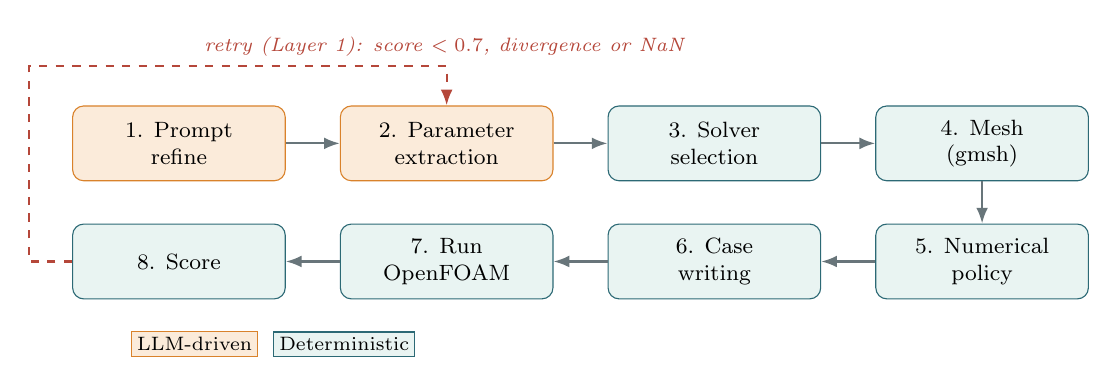
\begin{tikzpicture}[
  font=\footnotesize,
  stage/.style={rounded corners,draw=teal,fill=mint,minimum width=2.7cm,minimum height=0.95cm,align=center,inner sep=2pt},
  llm/.style={rounded corners,draw=orange,fill=lightorange,minimum width=2.7cm,minimum height=0.95cm,align=center,inner sep=2pt},
  arr/.style={-{Latex[length=2mm]},thick,draw=midgray},
  retry/.style={-{Latex[length=2mm]},thick,dashed,draw=alertred}
]
\node[llm]   (n1) at (0,0)     {1. Prompt\\refine};
\node[llm]   (n2) at (3.4,0)   {2. Parameter\\extraction};
\node[stage] (n3) at (6.8,0)   {3. Solver\\selection};
\node[stage] (n4) at (10.2,0)  {4. Mesh\\(gmsh)};
\node[stage] (n5) at (10.2,-1.5) {5. Numerical\\policy};
\node[stage] (n6) at (6.8,-1.5)  {6. Case\\writing};
\node[stage] (n7) at (3.4,-1.5)  {7. Run\\OpenFOAM};
\node[stage] (n8) at (0,-1.5)    {8. Score};
\draw[arr] (n1)--(n2); \draw[arr] (n2)--(n3); \draw[arr] (n3)--(n4);
\draw[arr] (n4)--(n5);
\draw[arr] (n5)--(n6); \draw[arr] (n6)--(n7); \draw[arr] (n7)--(n8);
\coordinate (rl) at ([xshift=-0.55cm]n8.west);
\coordinate (rt) at ([yshift=0.5cm]n1.north);
\draw[retry] (n8.west) -- (rl) -- (rl |- rt) -- (n2.north |- rt) -- (n2.north);
\node[font=\scriptsize\itshape,text=alertred,anchor=south west] at ([xshift=0.2cm]rt) {retry (Layer 1): score $<0.7$, divergence or NaN};
\node[draw=orange,fill=lightorange,font=\scriptsize,inner sep=2pt] at (0.2,-2.55) {LLM-driven};
\node[draw=teal,fill=mint,font=\scriptsize,inner sep=2pt] at (2.1,-2.55) {Deterministic};
\end{tikzpicture}

\vspace{-0.1cm}
\begin{columns}[T,onlytextwidth]
\column{0.48\textwidth}
\begin{block}{LLM only where needed}
\footnotesize Prompt refinement, parameter extraction, RAG context, retry generation.
\end{block}
\column{0.48\textwidth}
\begin{block}{Deterministic where correctness matters}
\footnotesize Solver routing, mesh generation, case writing, execution, scoring.
\end{block}
\end{columns}
\end{frame}

\begin{frame}{Pipeline walk-through: stages 1--4 (understand and mesh)}
\small
\renewcommand{\arraystretch}{1.25}
\begin{tabularx}{\textwidth}{>{\bfseries}l >{\bfseries}l L L}
\toprule
\# & Stage & What happens & Example \\
\midrule
1 & Prompt refine & LLM restates the request in a consistent, explicit form. & ``cavity re 150 water'' $\to$ lid-driven cavity, $Re=150$, water \\
2 & Parameter extraction & Schema-constrained LLM output fills \texttt{CFDParams}: geometry, $Re$, fluid, solver hints, turbulence model. & chord $=1$\,m, AoA $5^\circ$, $Re=10^6$ \\
3 & Solver selection & Deterministic rules on physics flags (transient, compressible, thermal, multiphase) pick one of 7 approved solvers. & compressible nozzle $\to$ \texttt{rhoSimpleFoam} \\
4 & Mesh (gmsh) & One of 13 parameterised geometry templates is meshed, with correct \texttt{polyMesh} boundary patches. & NACA airfoil mesh \\
\bottomrule
\end{tabularx}
\end{frame}

\begin{frame}{Pipeline walk-through: stages 5--8 (configure, run, judge)}
\footnotesize
\renewcommand{\arraystretch}{1.15}
\begin{tabularx}{\textwidth}{>{\bfseries}l >{\bfseries}l L L}
\toprule
\# & Stage & What happens & Why it matters \\
\midrule
5 & Numerical policy & Schemes, solvers and turbulence settings chosen for the flow regime (RANS only today). & Keeps numerics consistent with the physics \\
6 & Case writing & All dictionaries written deterministically, so boundary conditions agree across files. & Removes the invented-keyword failure mode \\
7 & Run OpenFOAM & The solver is executed; logs and residuals are captured. & Real execution is the ground truth \\
8 & Score & Reward $r\in[0,1]$ from convergence, residuals, solver choice, mass conservation, BC validity and penalties. & Drives retry and training-data selection \\
\bottomrule
\end{tabularx}
\vspace{0.15cm}
\begin{alertblock}{Retry loop (Layer 1)}
\footnotesize If the score is below $0.7$, or the run diverges or produces NaN, the pipeline retries with a corrected parameter set built from the solver log (RAG-augmented, or a surgical dictionary patch on localised errors).
\end{alertblock}
\end{frame}

\begin{frame}{Key design choices}
\begin{columns}[T,onlytextwidth]
\column{0.48\textwidth}
\begin{block}{Constrained parameter extraction}
\begin{itemize}\small
  \item \textbf{vLLM} for high-throughput inference.
  \item \textbf{xgrammar} JSON schema enforces the \texttt{CFDParams} structure, so output is always parseable.
  \item Output: geometry, $Re$, fluid, solver, turbulence model.
  \item Regex check of $Re=UL/\nu$ consistency between stated and derived values.
\end{itemize}
\end{block}
\column{0.48\textwidth}
\begin{block}{Deterministic solver routing}
\begin{itemize}\small
  \item Decouples solver choice from the LLM.
  \item Physics flags: transient, compressible, thermal, multiphase.
  \item Routes to one of \textbf{7 approved solvers}.
  \item Avoids LLM bias, e.g.\ \texttt{simpleFoam} for transient vortex shedding.
\end{itemize}
\end{block}
\end{columns}
\vspace{0.1cm}
\begin{block}{Design principle}
\small Use the LLM for language understanding; use rules and code wherever a wrong answer would crash a run or give a wrong physics set-up.
\end{block}
\end{frame}

\begin{frame}{The reward: how a run is scored}
\begin{columns}[T,onlytextwidth]
\column{0.52\textwidth}
\begin{block}{Positive terms}
\small
\renewcommand{\arraystretch}{1.15}
\begin{tabular}{@{}lr@{}}
\toprule
Criterion & Weight \\
\midrule
Convergence & 0.40 \\
Residual $<10^{-4}$ & 0.20 \\
Correct solver & 0.10 \\
Mass conservation & 0.05 \\
Valid boundary conditions & 0.05 \\
\bottomrule
\end{tabular}
\end{block}
\begin{alertblock}{Penalties (up to $-0.25$)}
\small Poor mesh quality, slow runtime, stagnation.
\end{alertblock}
\column{0.44\textwidth}
\begin{exampleblock}{How the score is used}
\small
\begin{itemize}
  \item $r<0.7$: trigger a retry.
  \item $r\ge0.5$: trajectory accepted into the foundational corpus.
  \item $r\ge0.65$: live run joins the training pool.
\end{itemize}
\end{exampleblock}
\begin{alertblock}{Known bias}
\small Reward favours convergence; a converged case can still be physically wrong (see limitations).
\end{alertblock}
\end{columns}
\end{frame}

\begin{frame}{Training data: static corpus + dynamic capture}
\begin{columns}[T,onlytextwidth]
\column{0.48\textwidth}
\begin{block}{Foundational knowledge corpus}
\begin{itemize}\footnotesize
  \item \textbf{402 rows} of expert OpenFOAM trajectories.
  \item 252 unique prompts across all solver types and geometries.
  \item Accepted trajectories: score $r\ge0.5$.
\end{itemize}
\end{block}
\column{0.48\textwidth}
\begin{block}{Dynamic trajectory capture}
\begin{itemize}\footnotesize
  \item Live production runs feed the dataset continuously.
  \item High-success runs ($r\ge0.65$) join the training pool.
  \item Currently \textbf{210 de-duplicated topologies}.
  \item Failed runs logged by type for DPO mining.
\end{itemize}
\end{block}
\end{columns}
\vspace{0.05cm}
\begin{exampleblock}{Out-of-distribution benchmark: 110 prompts (isolated from training)}
\centering\footnotesize
\begin{tabular}{lrr}
\toprule
\textbf{Solver family} & \textbf{Count} & \textbf{Share} \\
\midrule
\texttt{simpleFoam} (steady incompressible) & 74 & 67\% \\
\texttt{rhoSimpleFoam} (steady compressible) & 9 & 8\% \\
\texttt{interFoam} (multiphase VOF) & 7 & 6\% \\
Others (\texttt{pimpleFoam}, \dots) & 20 & 18\% \\
\bottomrule
\end{tabular}
\end{exampleblock}
\end{frame}

\begin{frame}{The seven-layer self-evolution loop}
\centering
\resizebox{\linewidth}{!}{%
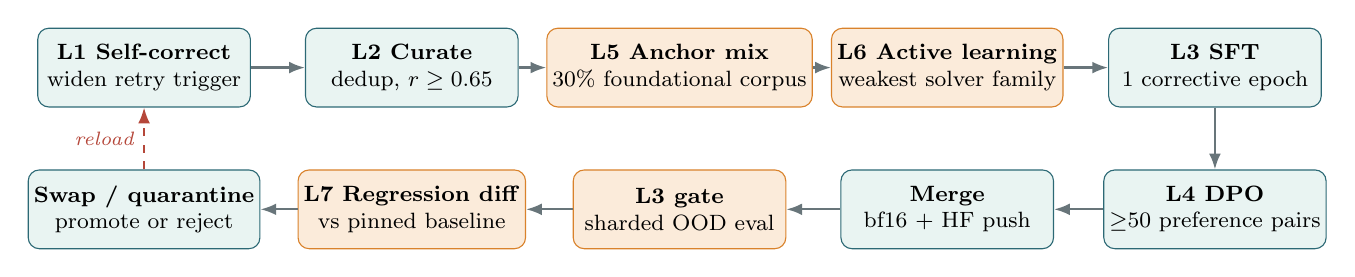
\begin{tikzpicture}[
  font=\footnotesize,
  layer/.style={rounded corners,draw=teal,fill=mint,minimum width=2.7cm,minimum height=1.0cm,align=center,inner sep=2pt},
  guard/.style={rounded corners,draw=orange,fill=lightorange,minimum width=2.7cm,minimum height=1.0cm,align=center,inner sep=2pt},
  arr/.style={-{Latex[length=2mm]},thick,draw=midgray}
]
\node[layer] (l1) at (0,0)    {\textbf{L1 Self-correct}\\widen retry trigger};
\node[layer] (l2) at (3.4,0)  {\textbf{L2 Curate}\\dedup, $r\ge0.65$};
\node[guard] (l5) at (6.8,0)  {\textbf{L5 Anchor mix}\\30\% foundational corpus};
\node[guard] (l6) at (10.2,0) {\textbf{L6 Active learning}\\weakest solver family};
\node[layer] (l3) at (13.6,0) {\textbf{L3 SFT}\\1 corrective epoch};
\node[layer] (l4) at (13.6,-1.8) {\textbf{L4 DPO}\\$\ge$50 preference pairs};
\node[layer] (mg) at (10.2,-1.8) {\textbf{Merge}\\bf16 + HF push};
\node[guard] (gt) at (6.8,-1.8)  {\textbf{L3 gate}\\sharded OOD eval};
\node[guard] (l7) at (3.4,-1.8)  {\textbf{L7 Regression diff}\\vs pinned baseline};
\node[layer] (sw) at (0,-1.8)    {\textbf{Swap / quarantine}\\promote or reject};
\draw[arr] (l1)--(l2); \draw[arr] (l2)--(l5); \draw[arr] (l5)--(l6); \draw[arr] (l6)--(l3);
\draw[arr] (l3)--(l4); \draw[arr] (l4)--(mg); \draw[arr] (mg)--(gt);
\draw[arr] (gt)--(l7); \draw[arr] (l7)--(sw);
\draw[arr,dashed,draw=alertred] (sw)--node[left,font=\scriptsize\itshape,text=alertred]{reload} (l1);
\end{tikzpicture}}

\vspace{0.1cm}
\begin{columns}[T,onlytextwidth]
\column{0.32\textwidth}
\begin{block}{L5: anchor mixing}
\scriptsize 30\% foundational corpus in every retraining batch prevents catastrophic forgetting.
\end{block}
\column{0.32\textwidth}
\begin{block}{L6: active learning}
\scriptsize Targets the weakest solver family and auto-generates new seeds for it.
\end{block}
\column{0.32\textwidth}
\begin{block}{L7: regression firewall}
\scriptsize Word-by-word diff against a pinned baseline before any weights are promoted.
\end{block}
\end{columns}
\vfill
\smallnote{Orange boxes mark safeguards; the diagram is a simplified linear view of the loop.}
\end{frame}

\begin{frame}{The seven layers in plain language}
\footnotesize
\renewcommand{\arraystretch}{1.2}
\begin{tabularx}{\textwidth}{>{\bfseries}c >{\bfseries}l L L}
\toprule
L & Name & What it does & Risk it addresses \\
\midrule
1 & Self-correct & Fixes failed runs from solver logs and retries. & Wasted failed runs \\
2 & Curate & Keeps only high-scoring ($r\ge0.65$), de-duplicated cases. & Learning from bad data \\
3 & Fine-tune + gate & One corrective SFT epoch, then test on held-out OOD prompts. & Shipping a worse model \\
4 & DPO & Learns from fail$\to$fix pairs: rejected failure vs chosen correction. & Repeating known mistakes \\
5 & Anchor mix & 30\% original corpus in every batch. & Catastrophic forgetting \\
6 & Active learning & Focuses on the weakest solver family; generates new seeds. & Uneven solver coverage \\
7 & Regression check & Diff against a pinned baseline before promotion. & Silent regressions \\
\bottomrule
\end{tabularx}
\end{frame}

\begin{frame}{Anti-collapse mechanisms}
\begin{block}{The self-distillation risk}
\footnotesize Training on self-generated data can quickly degrade quality. AutoFOAM uses \textbf{three complementary defences} plus a preference-learning layer.
\end{block}
\vspace{0.15cm}
\begin{columns}[T,onlytextwidth]
\column{0.32\textwidth}
\begin{exampleblock}{RAG-augmented retry}
\footnotesize Chroma vector DB of verified OpenFOAM tutorial configs; relevant dictionary snippets are injected into the retry prompt, grounding the fix in known-good files.
\end{exampleblock}
\column{0.32\textwidth}
\begin{exampleblock}{Surgical dictionary patching}
\footnotesize On localised \texttt{FOAM FATAL} errors only the offending dictionary is patched, skipping costly \texttt{gmsh} remeshing.
\end{exampleblock}
\column{0.32\textwidth}
\begin{exampleblock}{Prompt-diversity paraphrasing}
\footnotesize Varies the phrasing of training prompts so the model does not overfit one pattern.
\end{exampleblock}
\end{columns}
\vspace{0.2cm}
\begin{alertblock}{Layer 4: Direct Preference Optimisation (DPO)}
\centering\small
Failure trajectory (\emph{rejected}) $\longleftrightarrow$ Layer-1-corrected success (\emph{chosen})\\
DPO explicitly penalises the formulations that caused divergence.
\end{alertblock}
\end{frame}

\begin{frame}{Results: autonomous case generation}
\begin{columns}[T,onlytextwidth]
\column{0.52\textwidth}
\begin{block}{Coverage}
\begin{itemize}\small
  \item \textbf{7 solver families}, e.g.\ \texttt{simpleFoam}, \texttt{pimpleFoam}, \texttt{rhoSimpleFoam}, \texttt{interFoam}, \texttt{icoFoam}.
  \item \textbf{13 gmsh geometries}: cavity, step, NACA, cylinder, periodic hill, S-bend, Ahmed body, \dots
  \item Input: one natural-language sentence.
  \item Output: correct \texttt{polyMesh} boundaries and a convergent solution.
\end{itemize}
\end{block}
\column{0.44\textwidth}
\begin{exampleblock}{OOD headline metrics (110 prompts)}
\centering\small
\begin{tabular}{lr}
\toprule
\textbf{Metric} & \textbf{Value} \\
\midrule
FOAM FATAL-free & \textbf{110/110} \\
Execution success & \textbf{100\%} \\
Solver routing accuracy & \textbf{96.4\%} (106/110) \\
Mean reward $r$ & \textbf{0.64} \\
Geometry templates & \textbf{13/13} \\
Solver families & \textbf{7/7} \\
\bottomrule
\end{tabular}
\end{exampleblock}
\end{columns}
\vspace{0.1cm}
\begin{alertblock}{Misrouted: 4/110}
\footnotesize Ambiguous low-$Re$ cases only, e.g.\ transient cylinder at $Re=250$ $\to$ \texttt{icoFoam} (physically justifiable).
\end{alertblock}
\end{frame}

\begin{frame}{Representative OOD prompts}
\small
\renewcommand{\arraystretch}{1.25}
\begin{tabularx}{\textwidth}{l L l c}
\toprule
\textbf{Tag} & \textbf{Prompt} & \textbf{Predicted solver} & \textbf{Match} \\
\midrule
\texttt{cav\_re150}  & \emph{Cavity flow Re=150 in water, 0.4~m square} & \texttt{simpleFoam} & \checkmark \\
\texttt{pipe\_lam}   & \emph{Laminar pipe flow Re=500, diameter 0.02~m, water} & \texttt{simpleFoam} & \checkmark \\
\texttt{naca\_re1m}  & \emph{NACA0012 at Re=$10^6$, 5$^\circ$ angle of attack} & \texttt{simpleFoam} & \checkmark \\
\texttt{dam\_tall}   & \emph{Tall dam break, 2~m wide, 5~m water column collapse} & \texttt{interFoam} & \checkmark \\
\texttt{cdnoz\_ma04} & \emph{Convergent-divergent nozzle, Mach 0.4 throat, air} & \texttt{rhoSimpleFoam} & \checkmark \\
\texttt{cyl\_re250}  & \emph{Transient cylinder Re=250 in water, D=0.1~m} & \texttt{icoFoam} & $\times$ \\
\bottomrule
\end{tabularx}
\vspace{0.3cm}
\begin{block}{Evaluation infrastructure}
\small 8-way sharded cluster of \textbf{NVIDIA H100} GPUs; 110 OOD prompts kept isolated from training data.
\end{block}
\end{frame}

\begin{frame}{Autonomously generated meshes and flow solutions}
\centering
\begin{columns}[T,onlytextwidth]
\column{0.24\textwidth}\centering
\figbox{mesh-airfoil}{\linewidth}{1.9cm}{NACA mesh}\\[1mm]
\figbox{vel-airfoil}{\linewidth}{1.9cm}{NACA $|U|$}\\[1mm]
{\scriptsize NACA 4-digit airfoil}
\column{0.24\textwidth}\centering
\figbox{mesh-cylinder}{\linewidth}{1.9cm}{cylinder mesh}\\[1mm]
\figbox{vel-cylinder}{\linewidth}{1.9cm}{cylinder $|U|$}\\[1mm]
{\scriptsize Cylinder in cross-flow}
\column{0.24\textwidth}\centering
\figbox{mesh-periodic-hill}{\linewidth}{1.9cm}{periodic hill mesh}\\[1mm]
\figbox{vel-periodic-hill}{\linewidth}{1.9cm}{periodic hill $|U|$}\\[1mm]
{\scriptsize Periodic hill}
\column{0.24\textwidth}\centering
\figbox{mesh-sbend}{\linewidth}{1.9cm}{S-bend mesh}\\[1mm]
\figbox{vel-sbend}{\linewidth}{1.9cm}{S-bend $|U|$}\\[1mm]
{\scriptsize S-bend duct}
\end{columns}
\vfill
\begin{block}{}
\centering\small Top row: meshes. Bottom row: velocity magnitude. Each case came from a single natural-language prompt, with no manual intervention.
\end{block}
\end{frame}

\begin{frame}{Live demo: AutoFOAM web interface}
\begin{columns}[c,onlytextwidth]
\column{0.57\textwidth}
\centering
\href{https://www.youtube.com/watch?v=Kx17bfFlMSc}{%
  \figbox{demo-thumbnail}{\linewidth}{4.1cm}{Video thumbnail / screenshot of the AutoFOAM demo (click opens YouTube)}}
\column{0.40\textwidth}
\begin{block}{What the demo shows}
\begin{itemize}\small
  \item Natural-language prompt input.
  \item Automated parameter extraction.
  \item \texttt{gmsh} mesh generation.
  \item OpenFOAM case file synthesis.
  \item Live solver run and residual convergence.
  \item Field contours and one-click ParaView.
\end{itemize}
\end{block}
\begin{exampleblock}{Watch online}
\centering\small
\href{https://www.youtube.com/watch?v=Kx17bfFlMSc}{\texttt{youtu.be/Kx17bfFlMSc}}
\end{exampleblock}
\end{columns}
\end{frame}

\begin{frame}{What you get, and how to work with us}
\begin{columns}[T,onlytextwidth]
\column{0.48\textwidth}
\begin{block}{What you get}
\small
\begin{itemize}
  \item Hours of set-up cut to one prompt.
  \item Standard OpenFOAM cases you can inspect and edit.
  \item Python API, interactive REPL and batch runs.
  \item Self-hosted: one GPU ($\ge$24\,GB) + OpenFOAM v2412.
\end{itemize}
\end{block}
\column{0.48\textwidth}
\begin{block}{Extensible; work with us}
\small
The workflow can be extended to other CFD tools and to geometries of your choice.\\[3pt]
Pilots, custom solver/geometry extensions and commercial licensing.\\[3pt]
\scriptsize\texttt{github.com/AGN000/AutoFOAM}
\end{block}
\end{columns}
\end{frame}

% ============================================================
\section{Integration and outlook}
% ============================================================

\begin{frame}{How the pieces fit together (proposed workflow)}
\centering
\resizebox{\linewidth}{!}{%
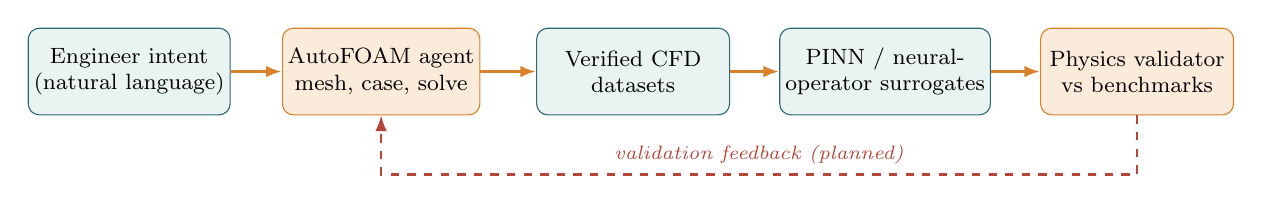
\begin{tikzpicture}[
  font=\footnotesize,
  box/.style={rounded corners,draw=teal,fill=mint,minimum width=2.45cm,minimum height=1.1cm,align=center,inner sep=2pt},
  agent/.style={rounded corners,draw=orange,fill=lightorange,minimum width=2.45cm,minimum height=1.1cm,align=center,inner sep=2pt},
  arr/.style={-{Latex[length=2mm]},very thick,draw=orange},
  fb/.style={-{Latex[length=2mm]},thick,dashed,draw=alertred}
]
\node[box]   (in)  at (0,0)    {Engineer intent\\(natural language)};
\node[agent] (ag)  at (3.2,0)  {AutoFOAM agent\\mesh, case, solve};
\node[box]   (ds)  at (6.4,0)  {Verified CFD\\datasets};
\node[box]   (sur) at (9.6,0)  {PINN / neural-\\operator surrogates};
\node[agent] (val) at (12.8,0) {Physics validator\\vs benchmarks};
\draw[arr] (in)--(ag); \draw[arr] (ag)--(ds); \draw[arr] (ds)--(sur); \draw[arr] (sur)--(val);
\draw[fb] (val.south) -- ++(0,-0.75) -| node[pos=0.25,above,font=\scriptsize\itshape,text=alertred]{validation feedback (planned)} (ag.south);
\end{tikzpicture}}

\vspace{0.4cm}
\begin{columns}[T,onlytextwidth]
\column{0.32\textwidth}
\begin{block}{Agent}
\small Removes the set-up barrier and produces verified, reproducible cases at scale.
\end{block}
\column{0.32\textwidth}
\begin{block}{Surrogates}
\small Physics-informed and geometry-aware models turn those cases into fast predictors.
\end{block}
\column{0.32\textwidth}
\begin{block}{Validator}
\small Benchmark checks catch solutions that converge numerically but are physically wrong.
\end{block}
\end{columns}
\vfill
\smallnote{Agent and surrogate results are shown separately in this talk; their coupling is a proposed direction.}
\end{frame}

\begin{frame}{Limitations and validation gaps}
\begin{columns}[T,onlytextwidth]
\column{0.48\textwidth}
\begin{alertblock}{Agentic CFD (AutoFOAM)}
\begin{itemize}\small
  \item \textbf{Geometry}: 13 parameterised gmsh models; no raw CAD (STEP/IGES).
  \item \textbf{Physics}: RANS only; no LES/DNS.
  \item \textbf{Reward}: biased toward convergence; a converged case can still be physically wrong (e.g.\ wrong drag coefficient).
  \item No cross-check against benchmark data (e.g.\ Ghia cavity).
\end{itemize}
\end{alertblock}
\column{0.48\textwidth}
\begin{alertblock}{Physics-informed surrogates}
\begin{itemize}\small
  \item One matched initialisation and two physics settings.
  \item Simplified crystal-growth PINN has no analytical reference.
  \item CFD cases are steady, laminar, axisymmetric, not industrial-scale melt flow.
  \item Velocity components can be much harder than temperature.
\end{itemize}
\end{alertblock}
\end{columns}
\vspace{0.2cm}
\begin{exampleblock}{Common remedy}
\small Add an external physics validator, and report component-level and field-wise errors rather than a single aggregate score.
\end{exampleblock}
\end{frame}

\begin{frame}{Research and validation roadmap}
\centering
\resizebox{\linewidth}{!}{%
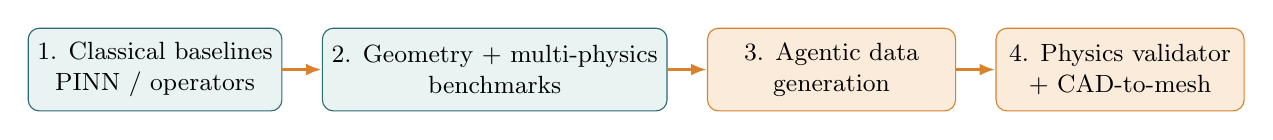
\begin{tikzpicture}[
  rstep/.style={rounded corners,draw=teal,fill=mint,minimum width=3.15cm,minimum height=1.05cm,align=center,font=\small},
  arr/.style={-{Latex[length=2mm]},very thick,draw=orange}
]
\node[rstep] (s1) {1. Classical baselines\\PINN / operators};
\node[rstep,right=0.5cm of s1] (s2) {2. Geometry + multi-physics\\benchmarks};
\node[rstep,right=0.5cm of s2,fill=lightorange,draw=orange] (s3) {3. Agentic data\\generation};
\node[rstep,right=0.5cm of s3,fill=lightorange,draw=orange] (s4) {4. Physics validator\\+ CAD-to-mesh};
\draw[arr] (s1)--(s2); \draw[arr] (s2)--(s3); \draw[arr] (s3)--(s4);
\end{tikzpicture}}

\vspace{0.4cm}
\begin{columns}[T,onlytextwidth]
\column{0.32\textwidth}
\begin{block}{Benchmark dimensions}
\small\begin{itemize}
  \item Accuracy, conservation, constraint satisfaction.
  \item Training / inference time.
  \item Data and memory needs.
\end{itemize}
\end{block}
\column{0.32\textwidth}
\begin{block}{Validation settings}
\small\begin{itemize}
  \item Silicon crystal growth.
  \item Turbulent-flow examples.
  \item Cryogenic / CFRP vessel examples.
\end{itemize}
\end{block}
\column{0.32\textwidth}
\begin{block}{Agentic extensions}
\small\begin{itemize}
  \item LES/DNS numerical policy.
  \item More solvers (\texttt{reactingFoam}, \texttt{chtMultiRegionFoam}).
  \item Tighter DPO feedback from the validator.
\end{itemize}
\end{block}
\end{columns}
\end{frame}

\begin{frame}{Key takeaways}
\begin{enumerate}\setlength{\itemsep}{3pt}\small
  \item \key{CFD acceleration is the driver:} high-fidelity multi-physics simulation is expensive and expertise-heavy.
  \item \key{PINNs add physics constraints:} PDEs, boundary and initial conditions become part of learning, but must be evaluated component by component: a smaller PDE residual (up to $\sim\!4800\times$ smaller) gave a \emph{worse} field.
  \item \key{Operators add generalisation:} PINO, PI-GANO and GAOT target solution families and geometries.
  \item \key{Surrogate error is field-specific:} temperature 5.6--9.6\% NRMSE, but axial velocity up to 41\%.
  \item \key{Agentic workflows remove the set-up barrier:} AutoFOAM reaches 100\% execution success and 96.4\% solver-routing accuracy on 110 OOD prompts.
  \item \key{Validation closes the loop:} physics validators and benchmark checks are essential for both surrogates and agents.
\end{enumerate}
\vfill
\centering
\large\textcolor{navy}{Physics + geometry + agentic automation}\\
\large\textcolor{midgray}{$\longrightarrow$ a coherent path toward accelerated CFD}
\end{frame}

% ============================================================
\section{References}
% ============================================================

\begin{frame}{Selected references}
\scriptsize
\begin{itemize}\setlength{\itemsep}{1.5pt}
  \item \emph{PINN review}, \url{https://doi.org/10.1063/5.0226232}.
  \item \emph{PI-GANO: physics-informed geometry-aware neural operator}, arXiv:2408.01600v1.
  \item \emph{Geometry Aware Operator Transformer (GAOT) / MAGNO}, arXiv:2505.18781v2.
  \item \emph{PINNsFormer: A Transformer-Based Framework for Physics-Informed Neural Networks} (2023), arXiv:2307.11833v3.
  \item D.\ Kolberg, C.\ Anders, S.\ Reke (2023), silicon VMCz crystal-growth PINNs, doi:10.1080/00219592.2023.2236656.
  \item J.\ Ling, Y.\ Zhang, D.\ Chen (2023), thermal--fluid coupling in silicon crystal growth, doi:10.1063/5.0123811.
  \item Y.\ Zhao, H.\ Liu, J.\ Xu (2025), thermal--fluid coupling in Czochralski silicon growth, doi:10.1063/5.0271778.
  \item N.\ Chapagain, R.\ Raj, B.\ K.\ Shine, A.\ A.\ S.\ (2026), \emph{Component-Level Evaluation of Adaptive PINN Training for CFD-Oriented Crystal Growth Simulation}, NeurIPS 2026 Sim2Science workshop.
  \item A.\ G.\ Neelan, A.\ Seshaditya, \emph{AutoFOAM: The Self-Refining Autonomous OpenFOAM Agent}.
  \item Related LLM-for-CFD work: FoamGPT, OpenFOAMGPT, Foam-Agent 2.0.
\end{itemize}
\vspace{0.1cm}
\textbf{Resources:}
\href{https://github.com/AGN000/AutoFOAM}{\texttt{github.com/AGN000/AutoFOAM}},
\href{https://github.com/AGN000/FoamAgentCases}{\texttt{github.com/AGN000/FoamAgentCases}},
\href{https://huggingface.co/arungovindneelan/foam-cfd-unified-14b}{\texttt{hf.co/arungovindneelan/foam-cfd-unified-14b}}
\end{frame}

% ============================================================ THANK YOU
\begin{frame}[plain]
\begin{tikzpicture}[remember picture,overlay]
  \fill[navy] (current page.south west) rectangle (current page.north east);
  \fill[teal] (current page.south east) rectangle ([xshift=-0.20\paperwidth]current page.north east);
  \fill[orange] ([xshift=-0.20\paperwidth]current page.south east) rectangle ([xshift=-0.195\paperwidth]current page.north east);
\end{tikzpicture}
\vspace{0.9cm}
\begin{minipage}{0.76\textwidth}
{\color{white}\fontsize{30}{36}\selectfont\bfseries Thank you\par}
\vspace{0.3cm}
{\color{white!85}\large A Seshaditya, QuaSi\par}
\vspace{0.25cm}
{\color{white!75}\small
With Arun Govind Neelan (AutoFOAM) and Niruta Chapagain, Rohit Raj,\\
Bertwin Kurisinkal Shine (crystal-growth PINNs)\\[2mm]
\href{https://quasi.digital}{quasi.digital}\quad
\href{https://github.com/adytiaa/quasi.ai}{github.com/adytiaa/quasi.ai}\quad
\href{https://adytiaa.github.io/quasi.ai/}{adytiaa.github.io/quasi.ai}\par}
\vfill
{\color{white!65}\small Physics-informed and agentic AI for accelerating CFD simulations\par}
\end{minipage}
\end{frame}

\end{document}
